%!TEX root = ../thesis.tex

%\begin{savequote}[70mm]
%	The Internet is becoming the town square for the global village of tomorrow.
%	\qauthor{Bill Gates}
%\end{savequote}


\chapter{Technologies}\label{chapter:technologies}
	
	This chapter explains more in detail the underlying technologies of this project.
	Starting from the general definition of a network and the most common architectures, to radio technologies work and then micro-controllers.
	
\section{Fundamentals of network communication}
	
	\begin{center}
		\begin{minipage}[H]{0.9\columnwidth}
			\begin{center}
				``\textit{A computer network is a structure that makes available to a data processing user at one place some data processing function or service performed at another place.}''~\cite{nla.cat-vn252493}
			\end{center}
		\end{minipage}
	\end{center}
	
	Starting from the definition of a computer network by Paul E. Green, it is easy to understand its importance in today's society.
	Smartphones, personal computers and other interconnected devices have become omnipresent in modern society, in which people need to feel connected to each other via these devices.
	% https://www.irishtimes.com/business/online-services-playing-more-important-role-in-everyday-activities-1.511857
	Not only they are used for fun, leisure and other social activities, but they allow connection to services such as online banking, government services and healthcare, that require a stable and secure connection among the systems that they use in order to provide a safe and sound experience for their users.
	All this to say, networks are everywhere underneath today's technology.
	There are no services or devices that can stand on their own without sharing data to other devices, to synchronize and provide a better user experience, to get updates from the manufacturer or simply to send a keep alive message.
	
	While this raw data is important for computers, people, the final users, process it to gain information, and this exchange of information from all around the world has brought radical changes many levels, from a cultural point of view to an economic point of view.
	The possibility of having a network of information exchange is the next step of globalization, which started with the exchange of goods among countries and now brings everyone together, allowing for a cultural exchange that lets people share and unite across the globe.
	
	This big network that is used to exchange information all around the world has a special name: Internet.
	% https://en.wikipedia.org/wiki/Right_to_Internet_access	
	% https://www.diplomacy.edu/blog/right-access-internet-countries-and-laws-proclaim-it/
	Many countries, such as Finland, Spain and Greece, have recognized the importance of this network and have given people the ''right to Internet access'', also known as the right to broadband or freedom to connect
	In these countries, service providers must be able to supply a mandatory minimum connection capability to all desiring home users in the regions of the country they serve.
	
	% http://www.redbooks.ibm.com/abstracts/gg243376.html
	It is important to note that Internet, with a capital I, is a particular set of worldwide interconnected networks \cite{gg243376}, but a common network of networks is called internetwork, shortened by internet, with a lowercase i.
	
	Such distinction began in the 1980s and has been described in RFCs \footnote{\href{https://datatracker.ietf.org/doc/html/rfc871}{RFC 871 (1982): A PERSPECTIVE ON THE ARPANET REFERENCE MODEL}}$^{,}$\footnote{\href{https://datatracker.ietf.org/doc/html/rfc872}{RFC 872 (1982): TCP-ON-A-LAN}} by computer scientists that understood how ARPANET was expanding and the its dimensions were not enough anymore to accommodate the amount of data traveling from one computer to another.
	% https://en.wikipedia.org/wiki/Commodore_64
	At that time, computers such as the IBM 5150 and the infamous Commodore 64 were starting to become more and more available, even if highly priced, not only to companies and universities, but also to consumers that brought them in their households, especially with the advent of MS-DOS, the dominant operating system throughout the 1980s and now open source \footnote{\url{https://github.com/microsoft/MS-DOS}}.
	
	As described by IBM in one of their technical books from the time, ''it is possible to divide the Internet such as the following groups of networks''\cite{gg243376}:
	\begin{itemize}[noitemsep]
		\item Backbones: large and strategical data routes among core networks and routers that compose and connect the Internet;
		\item Regional networks that connect large facilities such as universities and colleges;
		\item Commercial networks that provide to their subscribers access to the Internet;
		\item Local networks which run, for example, across a campus university;
	\end{itemize}

	\newpage

	% TODO sistemare posizione footnote alla fine
	% Oppure prendere mappa da https://www.globalbackbone.tisparkle.com/
	\begin{figure}
		\centering
		\includegraphics[width=\textwidth]{resources/img/chap3/backbone}
		\caption[Subsea Internet backbone cables between US and Europe.]{Subsea Internet backbone cables between US and Europe. \footnotemark}
	\end{figure}
	\footnotetext{~\url{https://www.infrapedia.com/app}}

	Given this increase of computers connecting to the Internet, there came the need for a revised structure that could better organize these components in a more robust, but also flexible, large network.

	With more accessible OSs, such as Windows 95 and Windows 98, and the advent of Tim Berners-Lee's World Wide Web (or WWW), computers became a commodity present in many households.
	The invention of the web and its ease to navigate, using hyperlinks and search engines, culminated in the dot com bubble, a stock market bubble in the late 90s that caused rapid rise of technology companies in stock market.
	
	Networks can be categorized based on the area they cover and serve:
	\begin{itemize}[noitemsep]
		\item Wide Area Network, or WAN: sometimes called long haul networks, provide communication over long distances;
		% https://www.cloudflare.com/learning/network-layer/what-is-a-metropolitan-area-network/
		\item Metropolitan Area Network, or MAN: provide communication inside a metropolitan area, which could be a single large city, multiple cities, or any given large area with multiple buildings;
		\item Local Area Network, or LAN: provide the highest speed connections among computers in a small and circumscribed area;
		% https://www.cloudflare.com/learning/network-layer/what-is-a-personal-area-network/
		\item Personal Ara Network, or PAN: connects devices within a user's immediate area.
	\end{itemize}

	In Sec. \ref{sec:radio_tech}, is described another level of distinction based on the power consumed by the transmission medium.
	
	Since everyone can connect to the Internet and access it's services, there is no need for the average user to understand what happens between his machine and the rest of the network, which means he only sees the information that is displayed to him without knowing where it arrives from or what path it took to arrive on his monitor.
	
	% inserire immagine con la nuvoletta che si vede dentro e non si vede dentro ?
	
	For computer scientists though, it is important to understand the difference between network architecture and network topology.	
	A network architecture, as described by by Paul E. Green, ``is a complete definition of all the layers necessary to build the network''\cite{nla.cat-vn252493}.
	This is focused on the network software, which needs to be highly structure in order to allow for heterogeneous systems to communicate with each other.
	% https://standards.iso.org/ittf/PubliclyAvailableStandards/s020269_ISO_IEC_7498-1_1994(E).zip
	One example of network architecture is the ISO/OSI reference model \footnote{\url{https://www.iso.org/standard/20269.html}}, which is implemented by the TCP/IP stack of protocols.

	\begin{figure}[H]
		\centering
		% https://stackoverflow.com/questions/38596488/in-which-layer-is-http-in-the-osi-model
		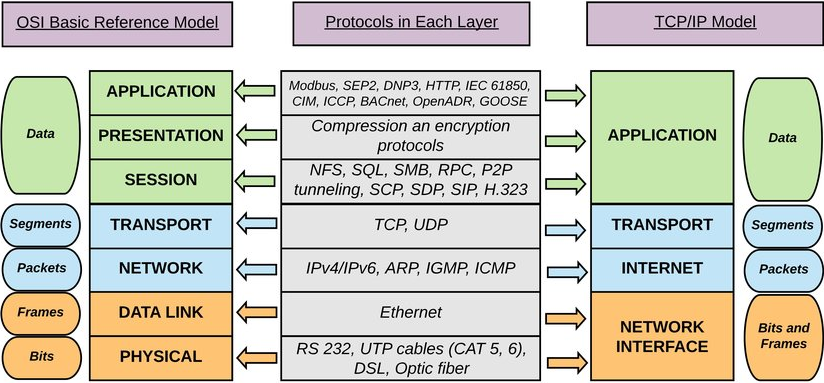
\includegraphics[width=\textwidth]{resources/img/chap3/isoosi}
		\caption{The ISO/OSI reference model against the TCP/IP stack}
	\end{figure}
	
	Thus comes the definition of a protocol as ``a set of agreements for interaction of two or more parties and is expressed by three components, syntax (e.g., a set of headers, a set of commands/responses), semantics (the actions and reactions that take place, including the exchange of messages), and timing, the sequencing and concurrency aspects of the protocol.''\cite{nla.cat-vn252493}.
	% TODO rivedere contenuto tra parentesi
	Different types of network use different architectures, based on the transmission medium and how well this performs (errors, speed, etc.).
	
	% https://www.omnisci.com/technical-glossary/network-topology
	On the other hand, the network topology refers to the manner in which the links and nodes of a network are arranged to relate to each other.
	
	\begin{figure}[H]
		\centering
		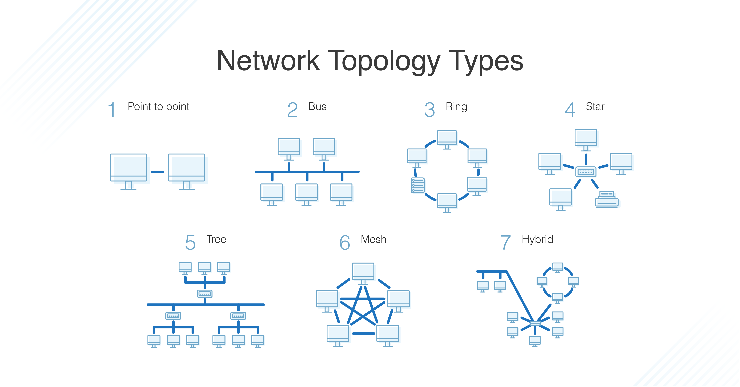
\includegraphics[width=\textwidth]{resources/img/chap3/network_topologies.png}
		\caption{Common network topologies}
		\label{img:network_topologies}
	\end{figure}
	
	As shown in Fig. \ref{img:network_topologies}, some of the most common network topologies are:
	\begin{itemize}[noitemsep]
		\item Point-to-Point: in which devices are connected directly;
		\item Bus: devices are connected to each other via a backbone cable;
		\item Ring: two dedicated point-to-point links connect a device to the two devices located on either side of it, creating a ring of devices through which data is forwarded via repeaters until it reaches the target device;
		\item Star: connects each device in the network to a central hub. Devices can only communicate with each other indirectly through the central hub;
		\item Tree: parent-child hierarchy in which star networks are interconnected via bus networks;
		\item Mesh: a dedicated point-to-point link connects each device on the network to another device on the network, only carrying data between two device;
		\item Hybrid: any combination of two or more topologies;
	\end{itemize}

	% TODO rivedere bene quando si scrive resto della tesi
	The project presented in this thesis regards a network with a mesh topology.
	This is better described in chap5 in a more depth and technical way
	The mesh proposed in this thesis has a span of LAN / MAN, since it connects devices that are in a circumscribed area but can be also placed further from each other, in order to cover longer distances.
	
	% TODO è necessaria?
	Another important distinction to make is the one between a distributed systems and a computer network.
	
	% COPIATO DA INTERNET: responsible for technical management of IETF activities and the Internet standards process
	Nowadays, the organization responsible for technical management of IETF activities and the Internet standards process is the Internet Engineering Steering Group (IESG)\footnote{\url{https://www.ietf.org/about/groups/iesg/}}.
	It is necessary to have an organization looking over the Internet itself since it gives the regulations that allow all devices to interconnect with each other.
	
	\newpage	

\section{Radio technologies}\label{sec:radio_tech}
	
	% TODO RIVEDERE PERCHé HAI COPIATO TROPPA ROBA DA WIKIPEDIA
	% https://en.wikipedia.org/wiki/Invention_of_radio
	Although Guglielmo Marconi is usually credited as the inventor of radio due to the creation of the first commercially successful wireless communication system, many scientists before him have studied radio waves.
	
	The idea of a wireless telegraph had been around for a while before the establishment of radio-based communication and scientist tried to achieve it via electric conduction and electromagnetic induction
	
	The discovery of electromagnetic waves, including radio waves, by Heinrich Rudolf Hertz in the 1880s came after theoretical development on the connection between electricity and magnetism that started in the early 1800s.
		
	
	
	Other important experiments were made by Nikola Tesla
	
	Tesla invented the Tesla coil during efforts to develop a "wireless" lighting system	
	Tesla employed the Tesla coil in his efforts to achieve wireless power transmission, his lifelong dream. 
	
	
	In order to give a complete picture of radio transmitting technologies, it is important to make a distinction among the ones that are made for internal or nearby use vs the ones that are used for longer distances.
	
	100 years later, radio technology has massively evolved and is used on a daily basis
	
	
	
	With new transmission technologies, new network architectures have emerged
	
	Topologies that bring computation closer to the edge are also rising, since they allow for faster computation and they bring data closer to the user
	
	LAN MAN and WAN are not enough anymore to describe the new topologies
	
	An important distinction is now made by other factors such as POWER, COST and RANGE of the transmiter receiver
	
	% TODO spiegare LPWAN
	
	Distinction of low cost vs higher cost
	% http://iotfactory.eu/iot-knowledge-center/overview-of-iot-networks/
	
	% PAPER : LPWAN Technologies: Emerging ApplicationCharacteristics, Requirements, andDesign Considerations
	\begin{figure}
		\centering
		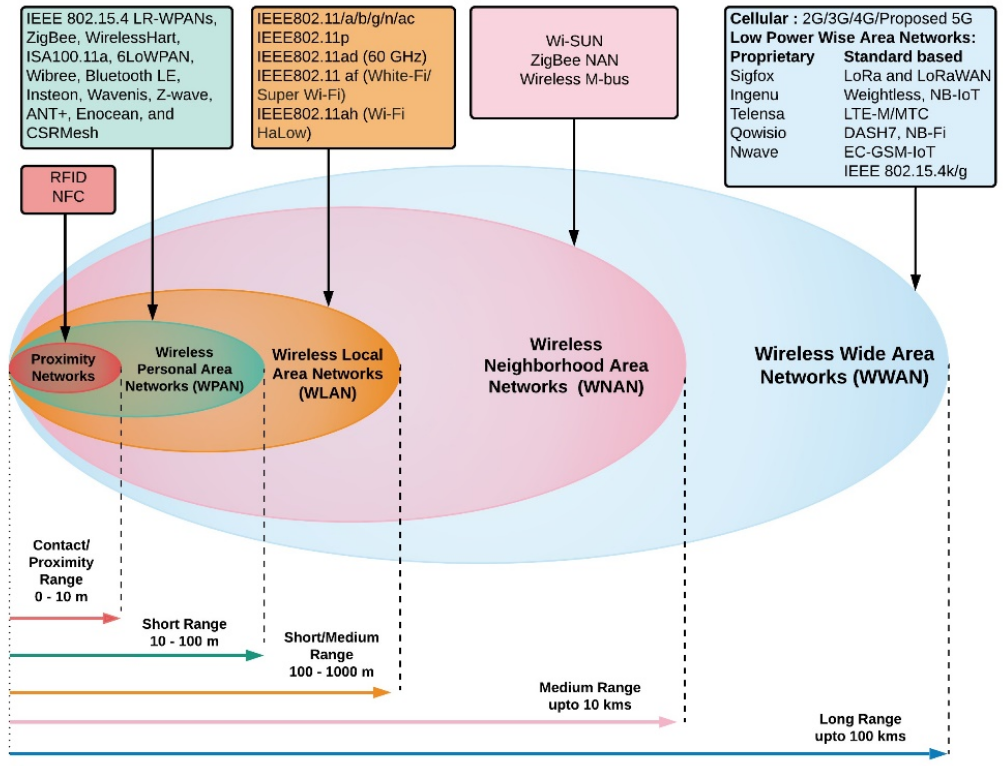
\includegraphics[height=\textwidth, angle=90]{resources/img/iot_range}
		\caption{}
	\end{figure}
		
	% https://www.sjsu.edu/faculty/watkins/transist.htm
	da quando Tesla e Marconi studiavano questa tecnologia, l'invenzione del transistor at the infamous bell labs e la miniaturizzazione del computer, come descritto anche in [fare riferimento al paragrafo dei microcontroller], hanno permesso di implementare questi mezzi trasmissivi a vaste categorie di dispositivi 
	
	Questo ha portato alla nascita dell'Internet of Things, o IoT, come descritto anche nel Chap2.
	
	Vengono descritte adesso alcune delle più importanti tecnologie radio per il mondo dell'iot

	Altre tecnologie sono RFID, ecc. ma quelle sono per un'altra storia
	
	\subsection{LoRa}
	
		https://lora-alliance.org/
		
		https://www.semtech.com/lora
		
		\begin{figure}
			\centering
			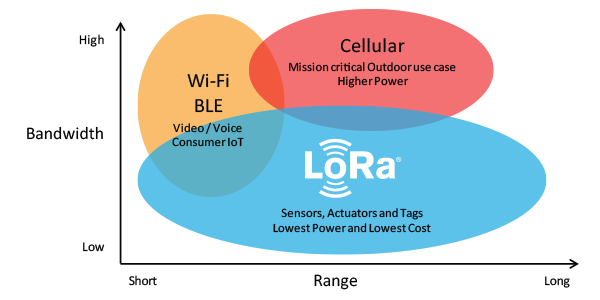
\includegraphics[width=\textwidth]{resources/img/LoRa_Why_Range}
			\caption{}
		\end{figure}
	
	
		The smaller the package, the greater the range.
		The greater the range, the fewer receiving antennas.
		The fewer antennas, the lower the total costs for the user.

	\subsection{LoRaWAN}
	
	\subsection{Bluetooth}		
	
	\subsection{WiFi}

	IEEE 802.11, better known in the public as WiFi, short for wireless fidelity
	
	\subsection{5G and LTE}
	
	The goal of fifth-generation (5G) wireless networks and beyond is to realize connecting “anything, anyone, anytime, anywhere” [1] reliably and energy-efficiently [ M. Agiwal, A. Roy and N. Saxena, "Next generation 5G wireless networks: A comprehensive survey", IEEE Communications Surveys \& Tutorials, vol. 18, no. 3, pp. 1617-1655, 2016.]
	

\section{LoRa and LoRaWAN}

\newpage
\newpage
	
\section{Hardware (Microcontrollers)}\label{sec:microcontrollers}

	Microcontrollers (or MCUs, short for Microcontroller Unit) are compact integrated circuits designed to govern a specific operation in an embedded system.
	They are specially made to fit in particular environments or to perform specific functions, which usually do not require any particular computation, memory capacity or power.
	This has been made possible thanks to the continuous shrinking of transistors, which makes almost all the components more compact, and the improved power sources.
	% TODO cambiare batteries con qualcos'altro?
	In junction with the previously described wireless technologies, microcontrollers are at the hearth of IoT devices, described in Chap. \ref{chap:background}, and they require long-lasting, low-cost, and sustainable batteries.
	
	% TODO modificare un attimo
	% TODO da riprendere in chap2
	% https://ieeexplore.ieee.org/abstract/document/9148855?casa_token=ppFhpgagThgAAAAA:u81u3jhRB-EJxsnQFx32i8LI4nJBKi3NsDvemcunZKNeSETGloW8wRB45S5OeaYOOdh2kXQ
	The number of IoT connected devices is expected to grow up to 75 billion worldwide by 2025 \cite{statista}, and connection density is expected to be one million devices per square km\cite{noma}.
	These devices will generate massive data and consume significant energy.
	
	Given the amount of specific functions an MCU can perform, there are many boards on the market.
	Some are very alike, while others are very different, since they are expected to be used in other types of environments.
	All boards consist on a similar architecture, which contains the processing unit (CPU), along with memory and programmable input/output peripherals.
	
	\begin{figure}[H]
		\centering
		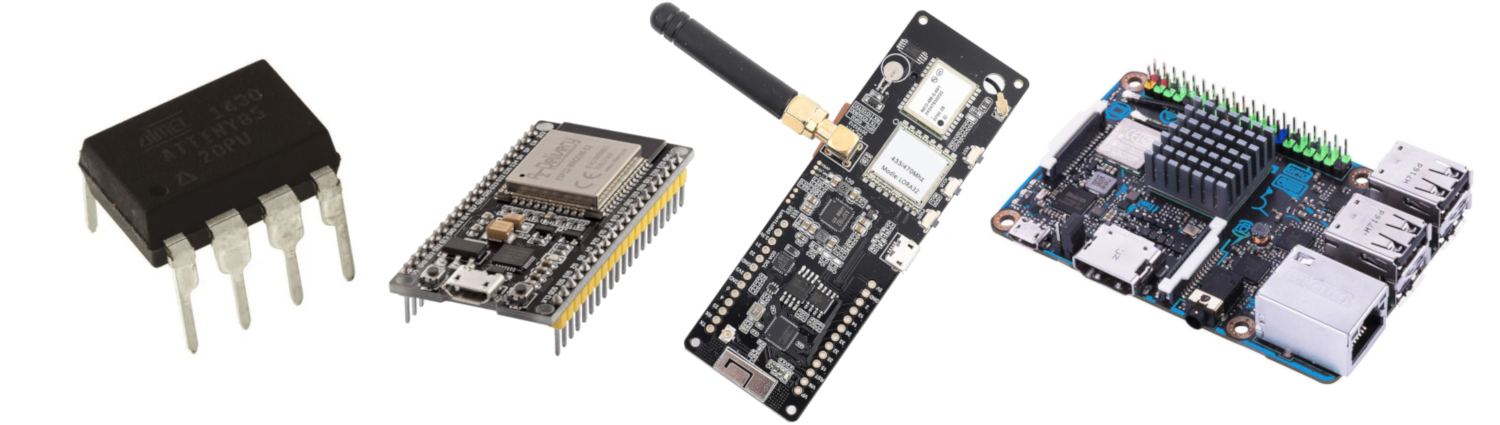
\includegraphics[width=\textwidth]{resources/img/chap3/generic_board}
		\caption{Attiny 85 on the left, in the middle two boards based on the ESP32, on the right the Asus Tinkerboard 2}
		\label{img:generic_board}
	\end{figure}

	% https://en.wikipedia.org/wiki/Microcontroller
	In Fig. \ref{img:generic_board}, there are four different boards, the one farthest on the left is the ATtiny 85 \footnote{\url{https://www.microchip.com/en-us/product/ATTINY85}}, a low-power, 8-bit microcontroller that is made for general purpose and can be programmed for simple tasks, from simple LEDs flashing, to more elaborate small sensor projects.
	% https://en.wikipedia.org/wiki/ESP32
	The two boards in the middle are based on the ESP32 chip, a series of low-cost, low-power system on a chip microcontrollers with integrated Wi-Fi and dual-mode Bluetooth.
	They both are more powerful than the ATtiny 85, and right one offers an integrated LoRa antenna on board.
	Far on the right, there is the Asus Tinkerboard 2 \footnote{\url{https://tinker-board.asus.com/product/tinker-board-2.html}}, a board powered by an Arm 6-core system on a chip (SoC), with a 64-bit Armv8 architecture.
	This board provides much more computing power compared to the previous ones and is able to run operating systems such as Linux and Windows.
	
	% https://www.amazon.it/Meipai-ATTINY85-20PU-ATTINY85-chip-ATMEL/dp/B08HPPMJ52/
	% https://www.amazon.it/AZDelivery-NodeMCU-Development-Arduino-gratuito/dp/B071P98VTG/
	% https://www.amazon.it/Scheda-Modulo-Wireless-T-Beam-Batteria/dp/B07X2KPN4L/
	% https://www.welectron.com/navi.php?qs=Tinker
	One of the strong points of these boards is the price: the ATtiny is priced around 1€ when bought in bulk, the boards on the middle cost around 7€ and 15€, while the board by Asus is the more expensive and starts from 70€.
	
	It is important to note though that using a generic board in a production environment might not be ideal, since it might lack of support and documentation.
	The boards described subsequently are from three of the major MCU producers, Arduino, Raspberry Pi and Pycom, which have built hardware that is well documented and suited for many different environments, from hobbysts to industrial use.

	\subsection{Arduino}
	
		% https://www.arduino.cc/en/Main/AboutUs
		% https://www.oreilly.com/library/view/arduino-a-technical/9781491934319/ch01.html	
		Arduino is a company founded by Massimo Banzi Et Al. in Ivrea, Italy, in 2005, and has released the first commercially available microcontroller.
		% TODO rivedere
		They wanted a device that was simple, easy to connect to various ''things'' (such as relays, motors, and sensors), and easy to program, besides being inexpensive.
		% It also needed to be inexpensive, as students and artists aren’t known for having lots of spare cash. 
	
		They selected the AVR family of 8-bit microcontroller devices from Atmel and designed a self-contained circuit board with easy-to-use connections, wrote bootloader firmware for the microcontroller, and packaged it all into a simple integrated development environment (IDE) that used programs called “sketches”. 
		Arduino was the result.
		
		The most famous version of their board is the UNO (one in English).
		Arduino UNO, the one on the left in Fig. \ref{img:arduino_board}, is the most used and documented board of the whole Arduino family.
		% https://www.circuito.io/blog/arduino-uno-pinout/
		Although this board does not have any integrated sensors or particular ports for peripherals.
		The current revision of the board is the Arduino UNO Rev 3 \footnote{\url{https://store.arduino.cc/products/arduino-uno-rev3}}, which consists of 14 digital pins, 6 analog inputs, a power jack, USB connection and ICSP header.
		
		% https://store.arduino.cc/products/arduino-uno-rev3
		% https://store.arduino.cc/products/arduino-yun-rev-2
		% https://store.arduino.cc/products/arduino-nano-33-ble
		\begin{figure}
			\centering
			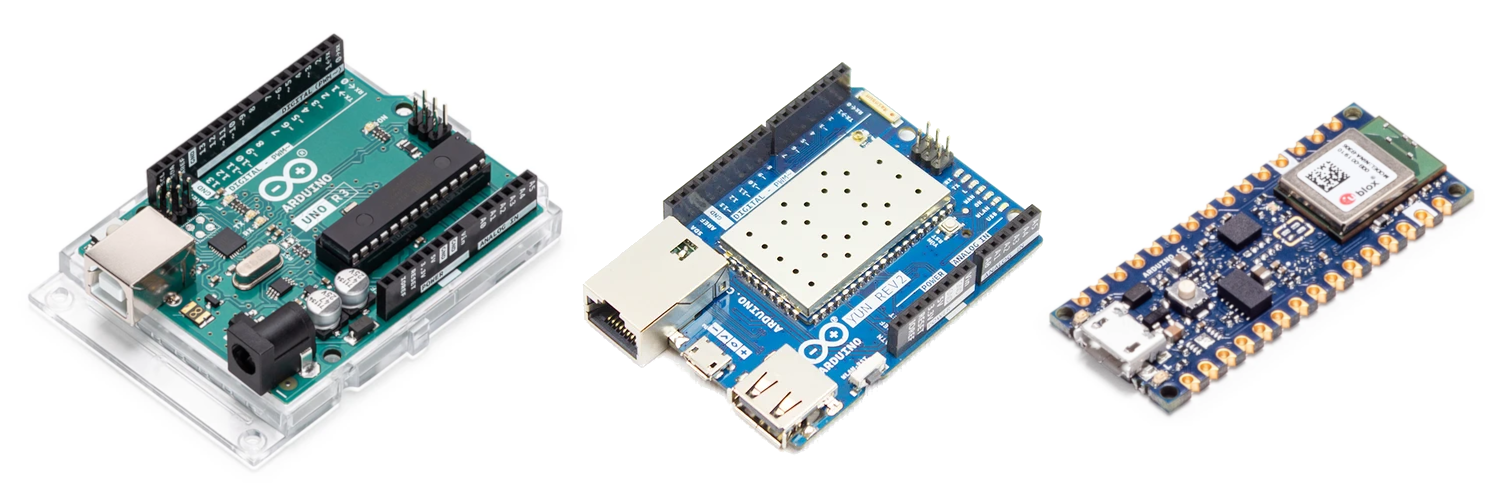
\includegraphics[width=\textwidth]{resources/img/chap3/arduino_types}
			% TODO rivedere accento yun, mettere link?
			\caption{Arduino UNO Rev 3 on the left, Arduino Yun in the middle, Arduino Nano 33 BLE on the right}
			\label{img:arduino_board}
		\end{figure}
		
		% https://www.circuito.io/blog/arduino-code/
		The Arduino family of products can be programmed in a particular programming language based on C/C++, using a special open-source integrated development environment (IDE).
		Arduino was so disruptive in the market that many boards, included the ones in Fig. \ref{img:generic_board}, support the Arduino C++.

		Shields are modular circuit boards that can be added to extend capabilities to different application needs.
		These can be attached directly on top of the board and provide sensors, interfaces, peripherals on a single board, rather than attaching to the Arduino singularly.
		% https://learn.sparkfun.com/tutorials/arduino-shields
		Some of the functionalities that can be added by a shield are Ethernet, WiFi, GPS, displays and cameras, motor drivers.
		
		The choice of making the Arduino schematics open-source and accessible to anyone has largely favored the development of newer boards, similar in capacity to the Arduino but more specialized, since producers and board makers are able to keep only the components needed or add different ones.
		An example can be the two middle boards in Fig. \ref{img:generic_board}, which rode the wave of Arduino's popularity.
		Not only the datasheets are available for all boards, but also the Arduino IDE software is open-source.
		
		% https://www.circuito.io/blog/arduino-code/
		The versatility of Arduino and its simple interface makes it a leading choice for a wide range of users around the world from hobbyists, designers, and artists to product prototypes. 
		
		Newer Arduino boards offer many integrated functionalities, for example:
		\begin{itemize}[noitemsep]
			% https://store.arduino.cc/collections/boards/products/arduino-mkr-nb-1500
			\item Arduino MKR NB 1500: offers an all-in-one solution for Narrowband IoT large-coverage solutions;
			% https://store.arduino.cc/collections/boards/products/arduino-mkr-wifi-1010
			\item Arduino MKR WiFi 1010: offers integrated WiFi and Bluetooth;
			% https://store.arduino.cc/collections/boards/products/arduino-nano-33-ble-sense
			\item Arduino Nano 33 BLE Sense: contains BLE connectivity and multiple sensors, such as 9 axis inertial, humidity, and temperature, barometric, microphone, gesture, proximity, light color and light intensity.
		\end{itemize}
	
		% TODO rivedere bene quando si scrive resto della tesi
		Particularly, this last model, the board on the right in Fig. \ref{img:arduino_board}, has been considered as one of the possible choices as development board for this project.
		As better explained in chap 5, it has been discarded since it does not offer LoRa connectivity and an additional module would have been necessary to connect the board in a mesh.
									
	\newpage
						
	\subsection{Raspberry Pi}
		
		The Raspberry Pi is a tiny and affordable computer that you can use to learn programming through fun, practical projects
		
		When compared to the Arduino, the Raspberry pi offers more functionalities, since it's architecture 
				
		% https://www.electronicshub.org/raspberry-pi-vs-arduino/
		Raspberry Pi and Arduino are two very popular boards among electronics DIY builders, hobbyists and even professionals. Raspberry Pi and Arduino are quite different boards. While Arduino is aimed at quick programming and circuit prototyping, Raspberry Pi acts as a learning tool for Computer Programming 
				
		The Raspberry Pi was developed by Eben Upton at the University of Cambridge in the United Kingdom with the aim of teaching and improving programming skills of students in developing countries. While Arduino is a Microcontroller based development board, the Raspberry Pi is a Microprocessor (usually an ARM Cortex A Series) based board that acts as a computer.
		
		You can connect several peripherals like a Monitor (through HDMI or AV Port), Mouse and Keyboard (through USB), connect to internet (through Ethernet or Wi-Fi), add a Camera (through the dedicated Camera Interface), just like we do to our desktop computer.
		
		Since the entire Computer (the Processor, RAM, Storage, Graphics, Connectors, etc.) is sitting on a single Printed Circuit Board, the Raspberry Pi (and other similar boards) are called as Single Board Computers or SBC.
		
		Another important thing about Raspberry Pi is, as it is a Linux based Computer, you can develop software using several Programming Languages like C, C++, Python, Java, HTML, etc.
		
		% --
		
		As the Arduino, there are different versions of raspberry pi, each one serving different scopes
		
		spiegare quali sono 
		
		% https://en.wikipedia.org/wiki/Raspberry_Pi
		\begin{figure}[H]
			\centering
			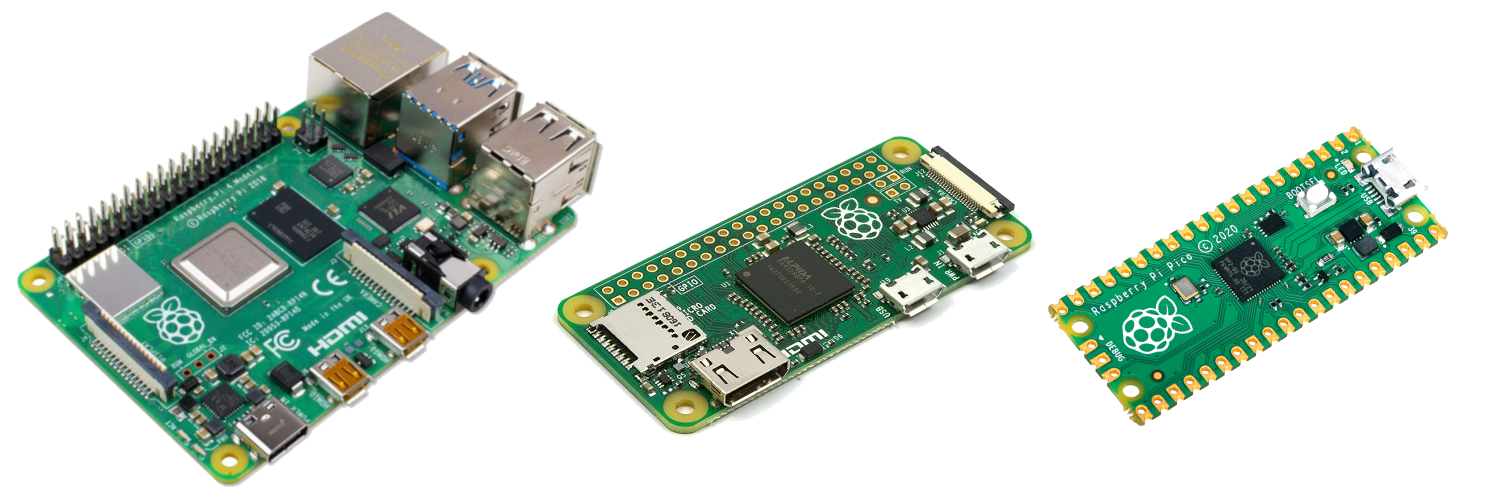
\includegraphics[width=\textwidth]{resources/img/chap3/raspberry_types}
			\caption{}
		\end{figure}
				
		Come mai non è stato scelto raspberry pi
			
		\newpage
			
	\subsection{Pycom}
	
%		\noindent
%		\begin{minipage}{0.5\textwidth}% adapt widths of minipages to your needs
%			
\includegraphics[width=\textwidth]{resources/img/pycom-logo-new-rp1}
%			\captionof{figure}{\textit{Pycom} company logo}
%		\end{minipage}%
%		\hfill%
%		\begin{minipage}{0.55\textwidth}\raggedright
%			Yesterday,\\
%			all my troubles seemed so far away\\
%			Now it looks as though they're here to stay\\
%			Oh, I believe in yesterday.				Yesterday,\\
%			all my troubles seemed so far away\\
%			Now it looks as though they're here to stay\\
%		\end{minipage}
		
		A Pycom development board has considerably more I/O than a standard Arduino, but probably comparable to an Arduino Mega. Easy to program via Python. Good example code from Pycom. Small community. Low cost. Not at all comparable to Raspberry Pi in terms of software flexibility.
		
		% https://www.reddit.com/r/IOT/comments/kx6knr/what_do_people_think_of_pycom_products/
		A complete LoRa gateway (Pygate + WiPy + IP67 box + antenna) costs around \$100, which is pretty good. So far very stable, and it was easy to configure. There's a PoE unit, but I use WiFi (at my home).

		Come mai sono state scelte le board di pycom per il progetto

		Mettere una tabella comparativa tra arduino raspberry e picom per dimostrare le capacità computazionali di ciascuno
		
		
		A more in depth description of how the chosen technologies interact is present in chap

		% https://pycom.io/product/fipy/
		
		\begin{figure}[H]
			\centering
			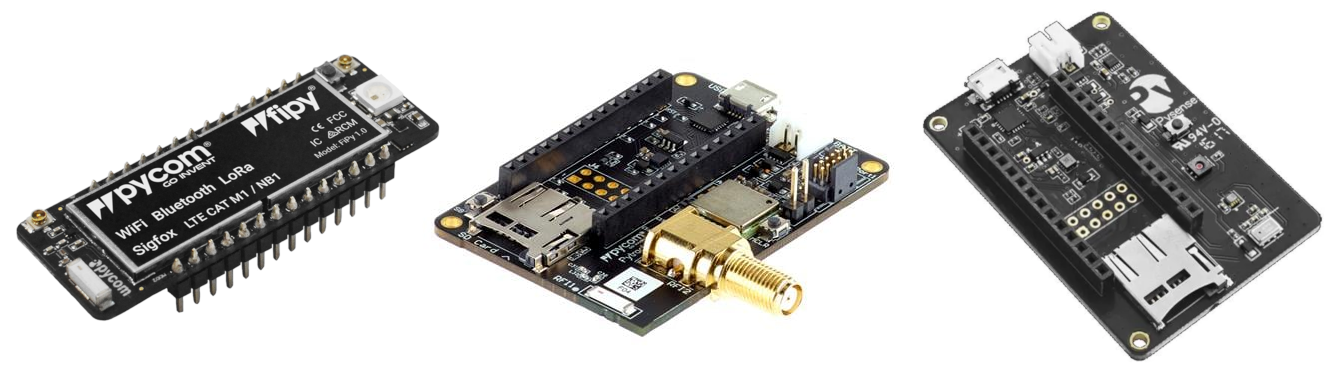
\includegraphics[width=\textwidth]{resources/img/chap3/pycom_board}
			\caption{}
		\end{figure}

		% TODO ADD TO REFERENCES
		% https://docs.pycom.io/gitbook/assets/lopy4-pinout.pdf
	